\documentclass[10pt]{article}
\usepackage[margin=.78in]{geometry}
\usepackage{amsmath,amssymb,booktabs,microtype,enumitem,graphicx,float}
\usepackage{hyperref}
\usepackage[T1]{fontenc}\usepackage{lmodern}
\setlist{nosep,leftmargin=*}
\title{The Inception of In-Context Learning:\\Minimal Training Structure for Contextual Candidate Promotion}
\author{Paper 0.8 --- Controlled ICL Mechanism Research Line}
\date{August 2026}
\graphicspath{{figures/}{docs/papers/paper0_8/figures/}}
\begin{document}\maketitle
\begin{abstract}
We ask for the smallest training structure and Transformer in which context promotes a target that is low-ranked without demonstrations to rank one. A leakage-audited D0--D4 ladder excludes the critical \(C\!\to\!3\) mapping and compares correct demonstrations with shuffled, wrong-chain, irrelevant, reversal, and no-context controls. A 54-cell coarse sweep finds 16 individual positives, including a one-layer, width-16, one-head model, but none of five Pareto-small candidates passes all three seeds. The closest D4 cells pass two of three seeds; failures arise either because the target is not promoted or because controls also solve the task. Thus D4 identifies a seed-sensitive acquisition frontier, not yet a stable general ICL mechanism. In parallel, contextual-copy calibration recovers a known microscopic circuit in one competent two-layer checkpoint: early pair binding, later associated-value transport, and rank-one promotion principally in second-layer attention. Value patching from shuffled context reduces accuracy from 100\% to 20.8\%, while demonstration-value ablation reduces it to 37.5\%. Fresh replications of the same copy architecture fail the 95\% three-seed gate, so this circuit is a validated local calibration rather than a stable minimality claim. The combined result separates the physical mechanism available after acquisition from the unstable conditions under which it appears.
\end{abstract}
\section{Question}
Let \(Y\) be a candidate with low context-free rank, \(\operatorname{rank}(Y\mid X)\gg1\). We seek the smallest training distribution \(\mathcal D^\star\) and smallest model \(M^\star\) for which \(\operatorname{rank}(Y\mid D_{\rm ctx},X)=1\), while \(Y\) remains low-ranked without \(D_{\rm ctx}\).
Define
\[
G_{\rm ICL}(Y)=m(Y\mid D_{\rm ctx},X)-m(Y\mid X),\quad
m(Y)=z(Y)-\max_{y\ne Y}z(y).
\]
The threshold is crossed when contextual margin becomes positive on held-out relations and the effect disappears under matched shuffled/wrong-context controls.

\section{Minimal motivating example}
Train local orders \(A\to B,B\to C\) and \(1\to2,2\to3\), but never train \(C\to3\) or the complete paired mapping. Test
\[
A\;1,\qquad B\;2,\qquad C\;?
\]
and ask whether context aligns the two local chains strongly enough to promote \(3\).

\section{Minimal-dataset ladder}
D0: random/no useful structure.\\
D1: isolated local successor chains only.\\
D2: many isomorphic independent chains.\\
D3: minimal paired/alignment exposure if D1--D2 fail.\\
D4: episode-specific random permutations preventing global mapping memorization.\\
D5: richer arbitrary/compositional relations only after the minimal mechanism is understood.

At each stage add exactly one structural ingredient.

\section{Dataset and model phase diagrams}
Search over number of relation families, examples per family, task/mapping entropy, chain length, symbol reuse, template variation, and position variation. Start with
\[
L\in\{1,2,3,4,6\},\qquad d_{\rm model}\in\{8,16,32,64\},
\]
and one or two heads where feasible. The goal is a behavioral phase boundary, not maximum benchmark performance.

\section{Controls}
Every positive cell compares no demonstrations, correct demonstrations, shuffled outputs, wrong-chain demonstrations, same-length irrelevant context, order perturbations, random initialization, held-out symbols, and held-out relation families. Audit that the critical direct mapping never occurs in training and that the target remains low-ranked without context.

\section{Layerwise mechanism}
At every boundary record residual state, SA update, FF update, target logit, rank, margin, top-$k$ candidates, and entropy. Compare context-free and context-conditioned trajectories. The first question is where \(Y\) becomes a serious candidate; the second is where it becomes rank one.

\section{Mechanistic hypotheses}
Test whether attention aligns corresponding relational roles, transports a successor/order state, or directly increases support for the target. Test whether FF already encodes reusable successor transformations, maps an attention-transported relation into the target direction, or simply sharpens a candidate. These are competing hypotheses.

\section{Causal experiments}
Ablate heads; zero or replace SA/FF updates; patch states from correct, shuffled, wrong, role-matched, and matched-norm controls; block individual demonstration tokens; and remove one local relation from training and retrain. Prefer causal loss of contextual promotion over attention-map interpretation.

\section{Before/after acquisition}
Find closely matched \(\mathcal D^-\) and \(\mathcal D^+\) conditions immediately below and above the ICL threshold. Compare head utility, SA/FF updates, residual target projection, relation-role similarity, cross-layer covariance, and weights. This threshold comparison is central.

\section{Minimality}
After finding a positive regime, delete one training family, relation type, positional regularity, symbol overlap, layer, head, or width. If the effect survives, simplify again.

\section{Interpretation}
Do not assume the Transformer is performing regression, Bayesian inference, or implicit gradient descent. Those may be useful behavioral approximations at larger scale. Prefer the smallest measured mechanism consistent with the evidence:
\[
\boxed{\text{learned local relations}+\text{contextual alignment/transport}+\text{candidate promotion}.}
\]

\section{D0--D4 behavioral results}
The reference L2/W32/H2 model was evaluated with three seeds. D0 never passes. D1 and D2 reach 87.5\% correct-context accuracy, but their controls can perform equally well; local order is therefore insufficient. D3 and D4 reach 100\% correct-context accuracy, yet only one of three seeds passes the complete context-dependence gate. Across the full 54-cell coarse surface, 16 cells pass individually.

\begin{figure}[H]\centering
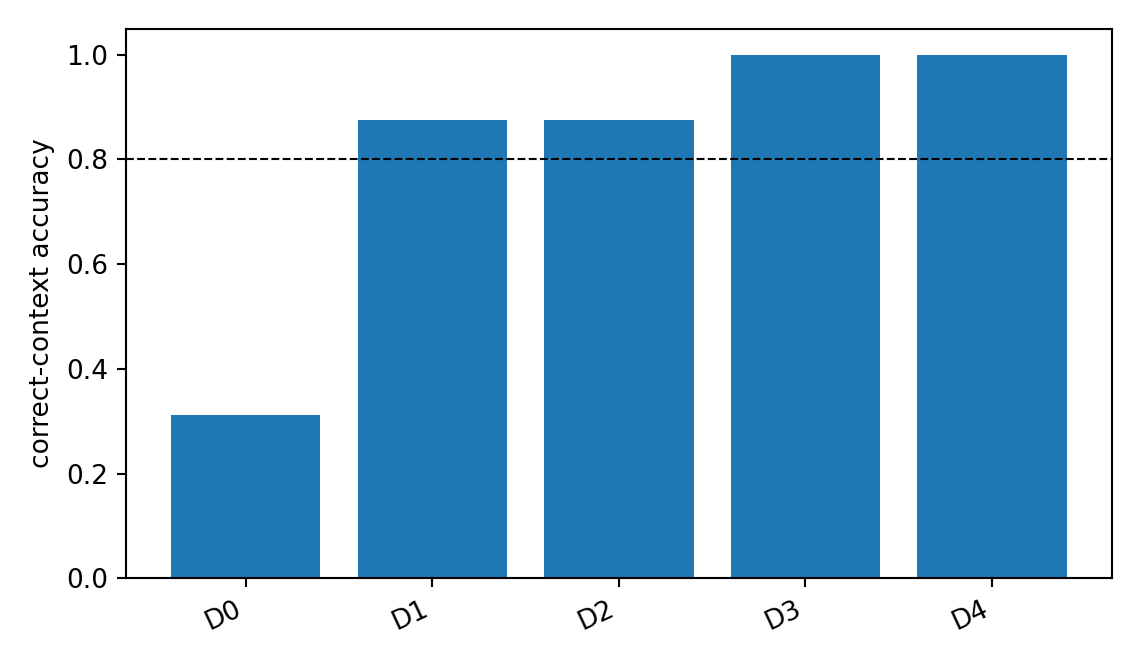
\includegraphics[width=.48\linewidth]{icl_dataset_phase_boundary.png}\hfill
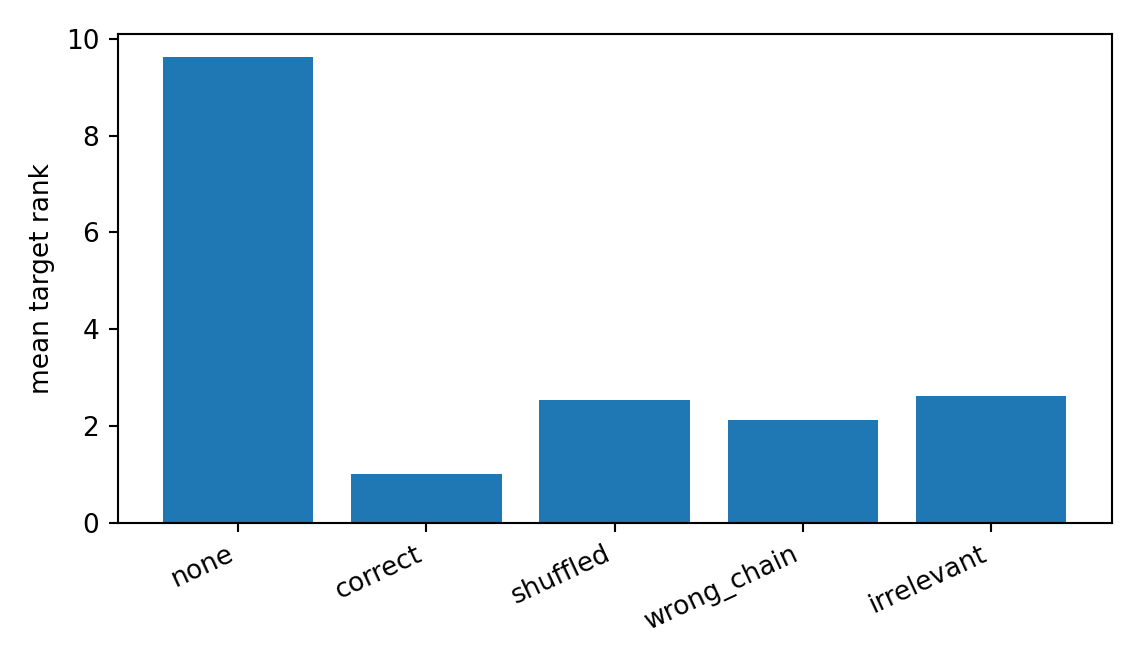
\includegraphics[width=.48\linewidth]{icl_context_free_vs_context_rank.png}
\caption{Left: dataset-ladder accuracy at the reference architecture. Right: D4 seed-11 rank promotion and matched controls. High correct-context accuracy is insufficient when a control also succeeds or the context-free target is already favored.}
\end{figure}

The smallest local positive is L1/W16/H1: 100\% correct context, zero context-free accuracy, mean context-free rank 26.5, zero negative-control accuracy, and margin gain 18.37. Replication rejects it: seeds 23 and 37 achieve only 25\%. Four further Pareto candidates also fail the three-seed gate. L2/W16/H1 and L6/W8/H1 pass two seeds; all others pass one. The supported result is a sharp, non-monotonic, seed-sensitive acquisition frontier. D4 tracing is consequently blocked rather than selected from a favorable seed.

\begin{figure}[H]\centering
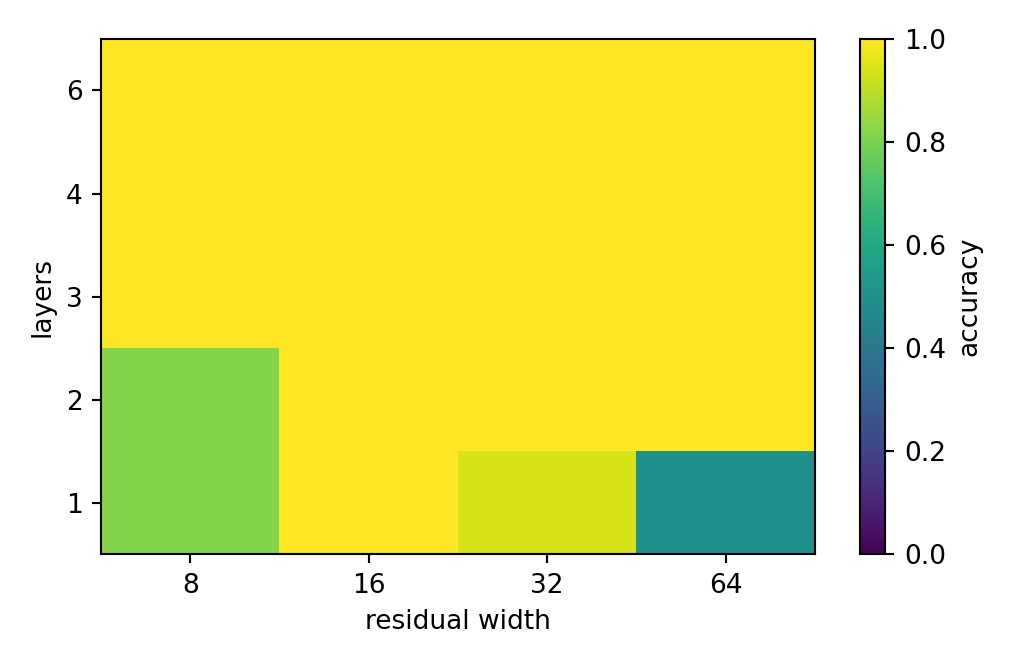
\includegraphics[width=.48\linewidth]{icl_model_phase_boundary.png}\hfill
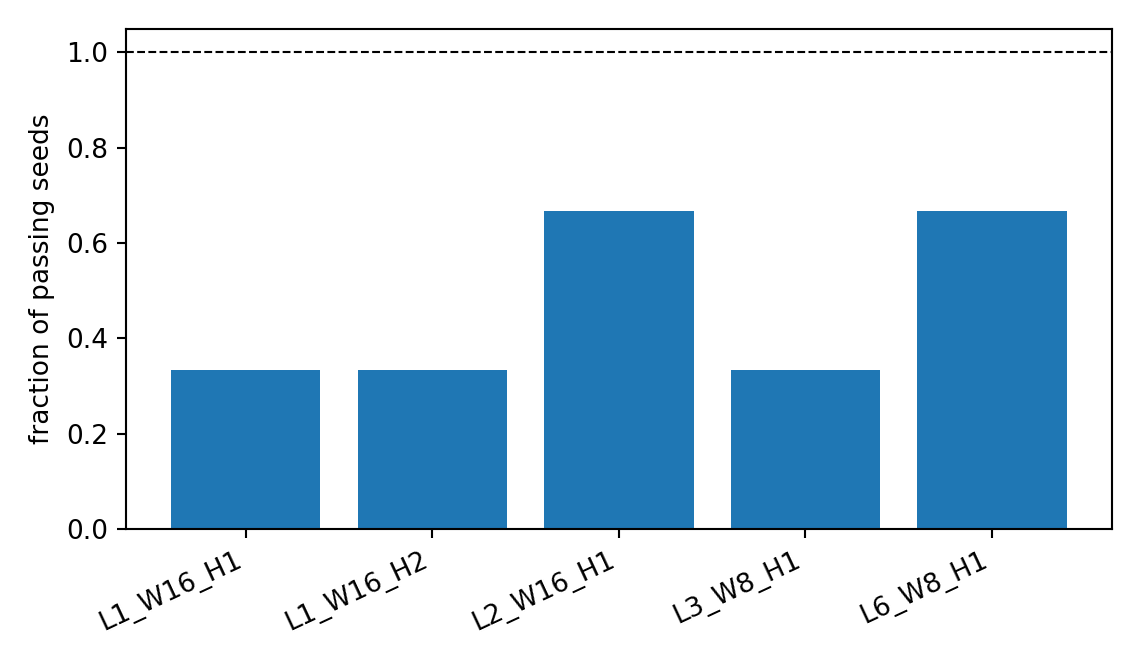
\includegraphics[width=.48\linewidth]{icl_before_after_acquisition.png}
\caption{Coarse seed-11 architecture surface (left) and three-seed replication fraction for Pareto-small positives (right). Deeper or wider models are not monotonically more selective.}
\end{figure}

\section{Contextual-copy calibration}
The C2 calibration uses balanced episode-specific associations, so a fixed key-to-value map cannot solve the query. One L2/W64/H2 checkpoint passes at 100\%, context-free rank 3.0, and 14.6\% maximum association-control accuracy. Exact Q/K/V tracing finds layer-0 head-0 previous-token mass 0.441. At layer 1, the two heads place 0.624 and 0.664 attention probability on the associated demonstration value, while repeated-key attention is only 0.039 and 0.068. This is a pair-binding then value-routing circuit, not a claim that attention probability itself is mass flow.

\begin{figure}[H]\centering
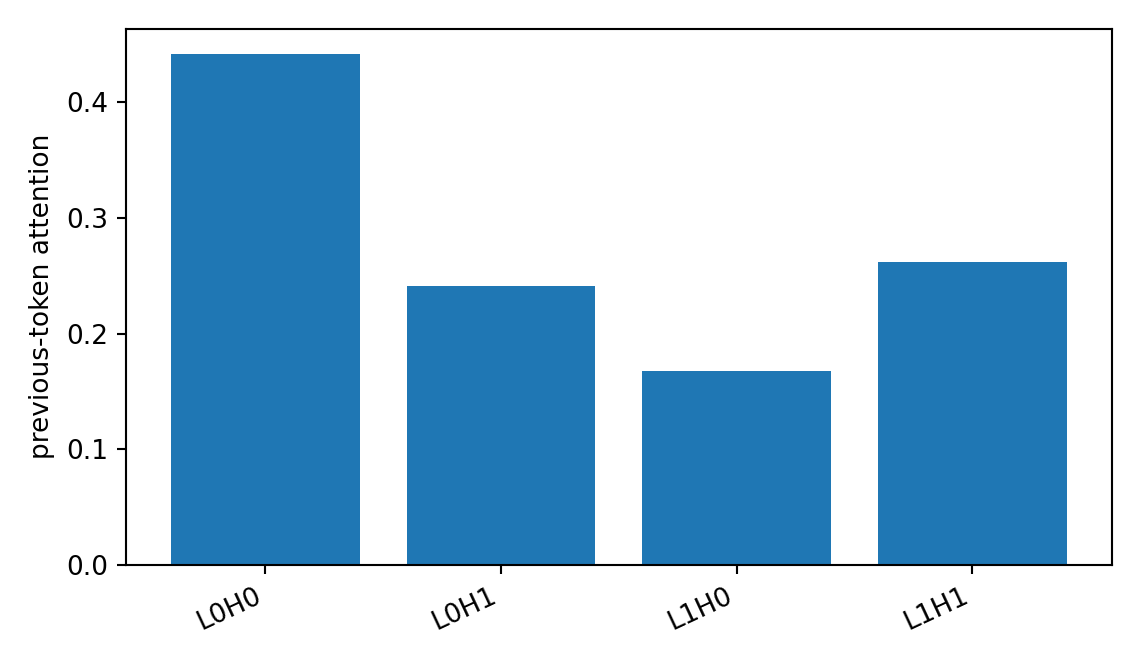
\includegraphics[width=.48\linewidth]{copy_qk_heatmaps.png}\hfill
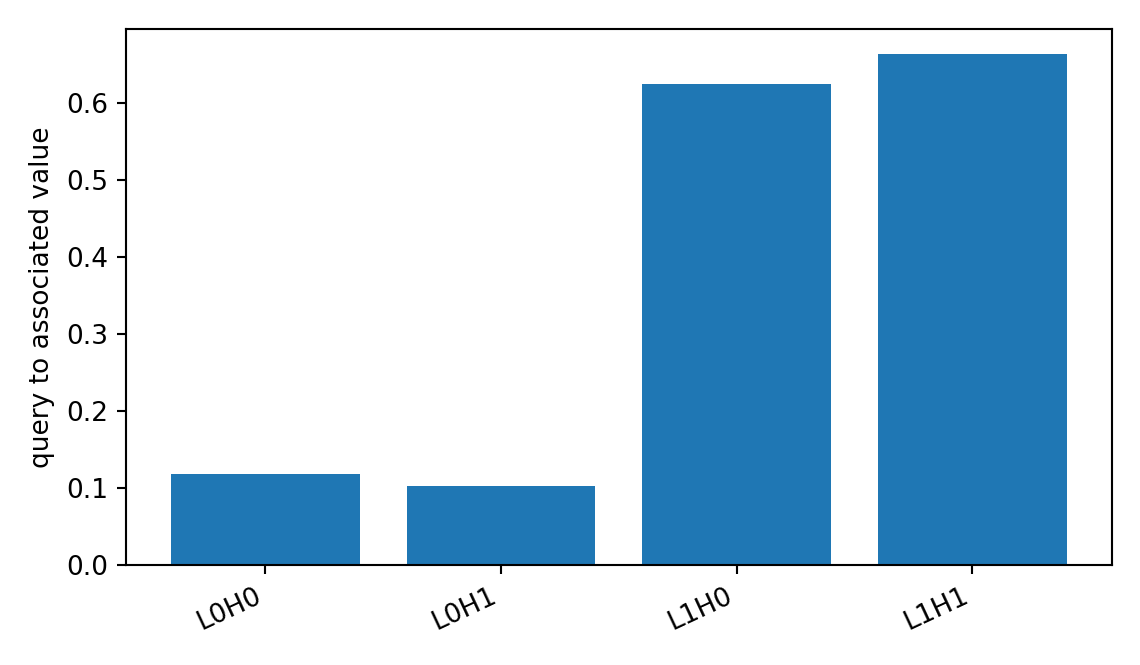
\includegraphics[width=.48\linewidth]{copy_attention_role_matrix.png}
\caption{Role-aligned copy calibration: early previous-token binding and later query-to-associated-value routing.}
\end{figure}

Causal tests agree. Layer-1 demonstration-value ablation lowers top-1 accuracy from 100\% to 37.5\% and damages margin by 15.24. Patching all layer-1 values from shuffled context lowers accuracy to 20.8\% (margin damage 24.89); patching keys retains 77.1\%. Layer-0 head-0 ablation lowers accuracy to 54.2\%, while both layer-1 heads are useful. Mean margin progresses from $-28.33$ initially through $-21.98$ after layer-0 SA and $-3.83$ after layer-0 FF, then to $+15.54$ after layer-1 SA. Final FF preserves rank one but slightly reduces margin to $+13.65$. Thus later attention supplies the decisive target support.

\begin{figure}[H]\centering
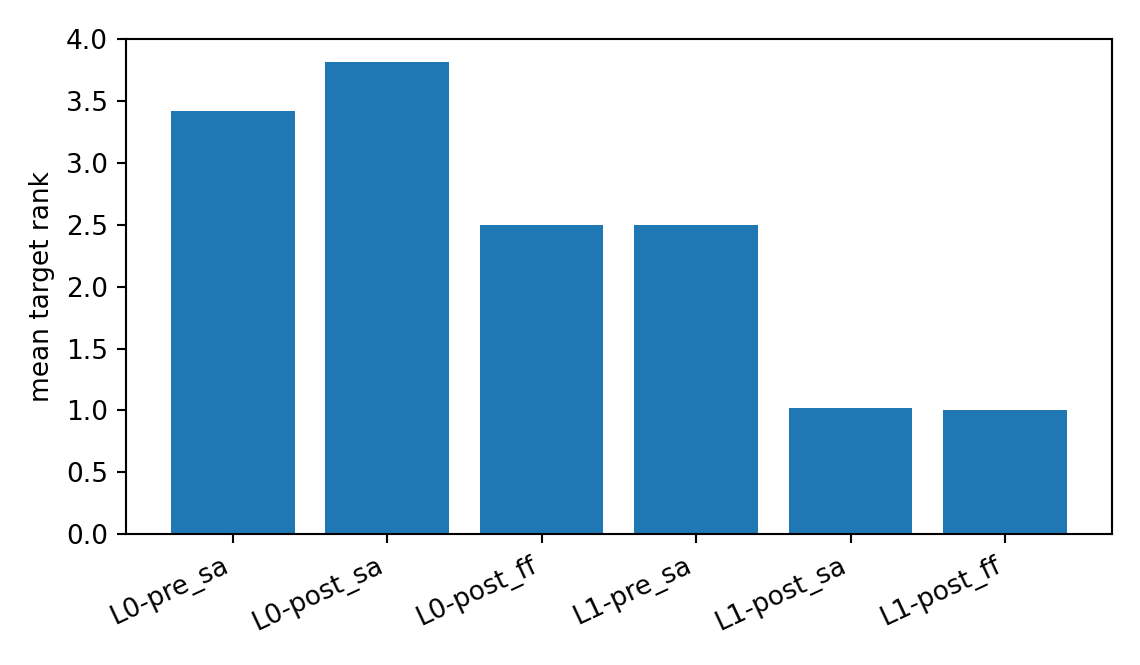
\includegraphics[width=.48\linewidth]{copy_target_rank_vs_depth.png}\hfill
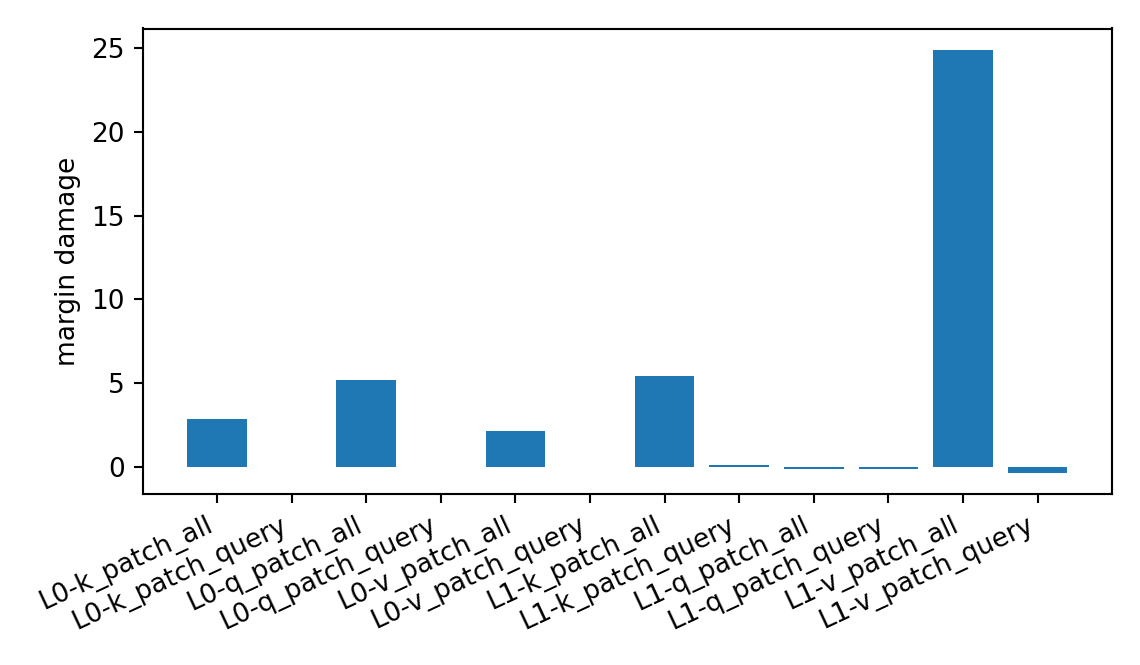
\includegraphics[width=.48\linewidth]{copy_qkv_patch_damage.png}
\caption{Target trajectory (left) and causal Q/K/V patch damage (right). The target becomes rank one principally in second-layer attention, and shuffled value transport is most destructive.}
\end{figure}

This is a local instrumentation calibration. Fresh L2/W64/H2 replications at 256 episodes reach 89.6\%, 70.8\%, and 66.7\%, all below the 95\% gate; L2/W128/H2 reaches only 41.7\%, 54.2\%, and 33.3\%. Increasing episode diversity to (E=1024) makes seeds 11 and 23 competent at both the nominal and doubled update budgets (100\% each), but seed 37 reaches only 52.1\% and 81.2\%, respectively. A targeted fourfold-budget run does not rescue seed 37: accuracy falls to 60.4\%. The non-monotonic trajectory rules out the simple explanation that this failure merely needed more updates. It instead supports an initialization- and optimization-sensitive acquisition boundary. Hence the circuit is physically validated where acquired, while reliable three-seed acquisition remains unestablished.

\begin{figure}[H]\centering
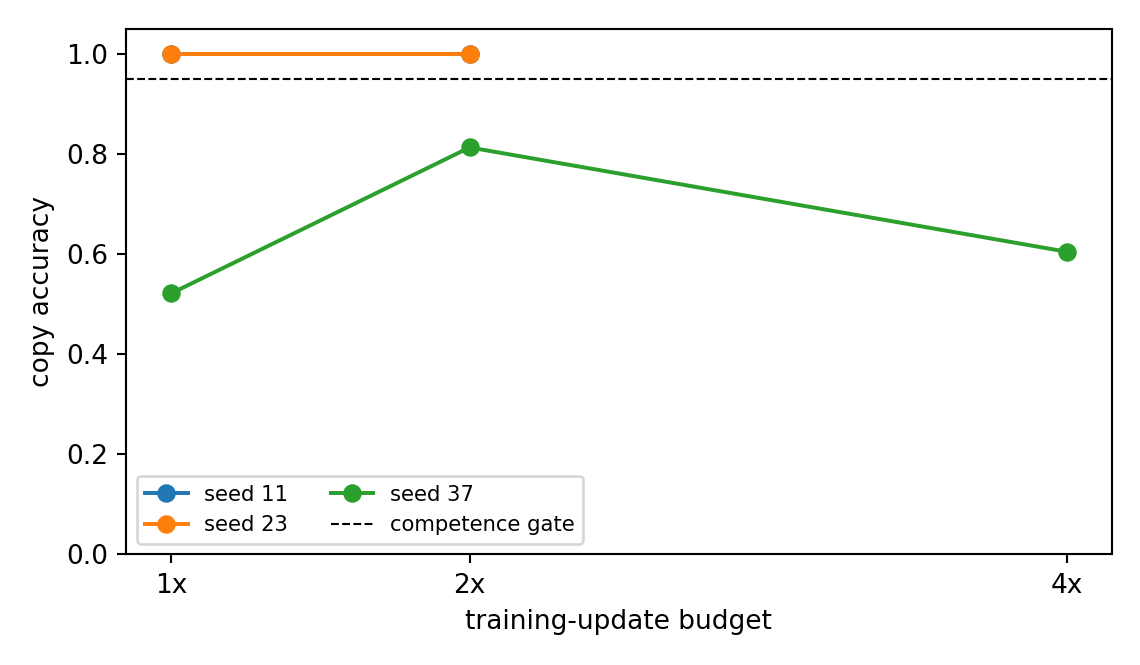
\includegraphics[width=.62\linewidth]{copy_before_after_acquisition.png}
\caption{Copy acquisition at (E=1024) versus update budget. Seeds 11 and 23 pass at the measured 1x and 2x budgets; seed 37 improves at 2x but regresses at 4x. The isolated 4x point is a targeted failure diagnostic, not a matched three-seed estimate.}
\end{figure}

\section{Answers and limitations}
Local order alone is not sufficient. Partial/fresh mapping pressure creates local positives, but no tested D4 architecture is seed-stable. Where contextual copy is acquired, the smallest measured mechanism is \emph{bind pairs, match the query role, transport the associated value, promote its logit}; second-layer SA is decisive and FF is supportive rather than the final promoter. Increasing copy diversity rescues two seeds, but update-budget scaling is non-monotonic for the remaining seed and does not close the replication gate. We find no need for regression, Bayesian, or implicit-gradient metaphors. We do not yet claim a stable smallest copy or D4 model, nor trace D4 from a selectively chosen seed. The next experiment should alter acquisition reliability---optimizer or curriculum, rather than update count alone---while keeping the leakage and control gates fixed.

\section{Reproducibility}
Generators and phase runners are under \path{src/cl/semantic/} and \path{src/cl/experiments/}. The shared tracer and analysis modules use the \path{paper08_*} prefix. Configurations are under \path{configs/paper08/}. Tracked artifacts include raw phase/control rows, five three-seed D4 replications, copy replication and exact trace tables, the (E=1024) training-budget diagnostic, compressed Q/K/V matrices, 18 figures, and summaries. Dense checkpoints remain locally reproducible and git-ignored.

\section{Relation to Papers 0.5--0.7}
Paper 0.5 studies predictive refinement once evidence is accessible. Paper 0.6 studies learned semantic/compositional relations. Paper 0.8 asks how context combines learned relations to create a new prediction without weight updates. Paper 0.7 remains deferred until these mechanisms justify synthesis.

\section{Scaling policy}
Do not scale merely to improve performance. Scale only if the minimal model cannot express the capability, a mechanistic hypothesis requires additional components, or external validity becomes the explicit question.

\section{Expected contribution}
\enlargethispage{2\baselineskip}
The target contribution is not another demonstration that Transformers perform ICL. It is an account of the \emph{inception} of ICL: the smallest statistical environment and neural architecture in which a frozen Transformer uses context to promote a prediction that its weights alone do not support, together with a causal account of where that probability mass comes from.
\end{document}
